\documentclass[a4paper]{article}

\usepackage[T2A]{fontenc} % Поддержка кириллических шрифтов T2A
\usepackage[utf8]{inputenc} % Кодировка исходного файла UTF-8
\usepackage[russian]{babel} % Правила переносов и названия для русского языка
\usepackage{graphicx}
\usepackage{float}
\usepackage{hyperref} % Для ссылок
\usepackage{amsmath, amssymb} % Математические символы и окружения
\usepackage{caption}
\usepackage{geometry}
\usepackage[normalem]{ulem} % Для \uline, \uuline и т.д. (если нужно)
\usepackage{mathtools} % Расширение для amsmath
\usepackage{siunitx} % Для красивой записи единиц измерения (\SI)

\geometry{top=2cm,bottom=2cm,left=2cm,right=2cm} % Поля страницы

\DeclareSIUnit\calorie{кал} % Определение калории, если потребуется

\date{} % Убираем дату

\begin{document}

\begin{center}
\textsc{Санкт-Петербургский национальный исследовательский университет информационных технологий, механики и оптики\\[3mm] % Изменено: ИТМО -> Университет ИТМО
Физический факультет}
\end{center}
\vspace{5mm}
\line(1,0){\textwidth}
\begin{center}
\textbf{ЛАБОРАТОРНАЯ РАБОТА № 2.05}\\[2mm] % Убран лишний \\, добавлен отступ
\textbf{Определение удельной теплоты кристаллизации и изменения энтропии при охлаждении олова} % Убраны кавычки
\end{center}
\vspace{2mm}
\line(1,0){\textwidth}
\vspace{5mm}
\begin{minipage}{0.4\textwidth}
    Группа: \textbf{Z3144} \\ % Укажите вашу группу
    Студент: \textbf{Евгений Турчанин}\\ % Укажите ваше имя
    \vspace{1mm}
\end{minipage}
\hfill % Чтобы растянуть пространство до правого края (если нужно)
\vspace{1mm}
\line(1,0){\textwidth}

\section{\textbf{Цель работы}}

\begin{itemize}
    \item Определение изменения энтропии при фазовом переходе первого рода на примере кристаллизации олова из расплава при его охлаждении.
    \item Определение теплоты кристаллизации олова на основе закона сохранения энергии.
\end{itemize}

\section{\textbf{Задачи}}

\begin{enumerate}
    \item Провести прямые измерения показаний милливольтметра, фиксирующего термоЭДС в процессе охлаждения олова.
    \item Построить график зависимости температуры олова от времени.
    \item Вычислить удельную теплоту кристаллизации и изменение энтропии олова при кристаллизации.
    \item Оценить погрешности измерений и сравнить полученные результаты с табличными значениями.
\end{enumerate}

\section{\textbf{Теоретическое введение}}

Кристаллизация – процесс перехода вещества из жидкого состояния в твердое.

Это один из фазовых переходов первого рода. \textbf{Фазовые переходы первого рода} (плавление, испарение) сопровождаются теплотой перехода, это то количество теплоты, которое необходимо сообщить веществу, чтобы изотермически – изобарически перевести его из одной фазы в другую. Фазовые переходы второго рода происходят без теплообмена. Это, например, изменение кристаллической модификации, переход в сверхпроводящее состояние, в сверхтекучее состояние у жидкого гелия, переход ферромагнетика в парамагнетик.

Процесс кристаллизации связан с выделением количества теплоты, равного теплоте плавления. Для химически чистых веществ процесс кристаллизации протекает при постоянной температуре, равной температуре плавления. В процессе кристаллизации упорядочивается движение частиц жидкости, постепенно прекращается перемещение молекул, возникают связанные тепловые колебания относительно узлов кристаллической решетки.

Для начала кристаллизации необходимо, чтобы в жидкости имелись центры кристаллизации – неоднородности, вокруг которых начинается процесс образования твердой фазы. Если в жидкости отсутствуют центры кристаллизации, то она может быть охлаждена до температуры более низкой, чем температура кристаллизации. В обычных условиях это, как правило, не происходит.

Количество теплоты, которое необходимо отвести от единицы массы жидкости при температуре кристаллизации для перехода жидкости в твердое состояние, называется удельной теплотой кристаллизации $\lambda$. Из первого начала термодинамики
\begin{equation} \label{eq:1}
-\lambda M_0 = U_{\text{тв}} - U_{\text{ж}} + p(V_{\text{тв}} - V_{\text{ж}})
\end{equation}
Здесь $U_{\text{тв}}, U_{\text{ж}}$ – внутренняя энергия вещества в твердом и жидком состоянии; $V_{\text{тв}}$ и $V_{\text{ж}}$ – объем твердой и жидкой фазы соответственно; $p$ – давление в процессе кристаллизации. Поскольку при переходе из жидкого в твердое состояние объем олова практически не меняется, имеем
\[
p(V_{\text{тв}} - V_{\text{ж}}) \ll U_{\text{тв}} - U_{\text{ж}}
\]
В этом случае
\begin{equation} \label{eq:2}
-\lambda M_0 = U_{\text{тв}} - U_{\text{ж}}
\end{equation}
Энтропия – функция состояния термодинамической системы.
Изменение энтропии в равновесном процессе равно отношению количества теплоты, сообщенного системе, к её температуре:
\begin{equation} \label{eq:3}
\delta S = \frac{\delta Q}{T}.
\end{equation}
Приращение энтропии при обратимом процессе
\begin{equation} \label{eq:4}
S_2 - S_1 = \int_{1}^{2} \frac{\delta Q}{T}.
\end{equation}
В процессе кристаллизации температура олова остаётся постоянной. При этом количество теплоты, отданное окружающей среде, равно
\begin{equation} \label{eq:5}
Q = \lambda M_0,
\end{equation}
где $M_0$ – масса олова. Так как $Q$ – количество теплоты, полученное системой от окружающей среды, то $Q = -\lambda M_0$. Из \eqref{eq:3} и \eqref{eq:4} следует, что
\begin{equation} \label{eq:6}
S_2 - S_1 = -\frac{\lambda \cdot M_0}{T_{\text{кр}}} = \frac{U_{\text{тв}} - U_{\text{ж}}}{T_{\text{кр}}} \cdot M_0.
\end{equation}
В процессе кристаллизации происходит упорядочение структуры вещества, внутренняя энергия системы уменьшается, что и приводит к убыванию энтропии.

\subsection*{Вывод расчетных формул}

Простейшей моделью охлаждения тела является охлаждение в среде с постоянной температурой $T_0$ (в термостате). Если процесс охлаждения происходит достаточно медленно, температуру произвольной точки тела в каждый момент времени можно считать одинаковой. Такой процесс охлаждения состоит из непрерывно следующих друг за другом равновесных состояний и, следовательно, является квазистатическим обратимым процессом. Применим закон сохранения энергии к квазистатическому процессу охлаждения твердого олова после кристаллизации, тогда для любого значения температуры твердого олова $T_i$:
\begin{equation} \label{eq:7}
(c_0 M_0 + c_A M_A) \cdot dT_i + \alpha \cdot S_A \cdot (T_i - T_0) \cdot dt = 0.
\end{equation}
Здесь $(c_0 \cdot M_0 + c_A M_A) \cdot dT_i < 0$ – количество теплоты, отданное телом среде при его охлаждении за малый интервал времени $dt$; $\alpha \cdot S_A \cdot (T_i - T_0) \cdot dt > 0$ – количество теплоты, полученное окружающей средой через поверхность ампулы площадью $S_A$ за время $dt$; $c_0, c_A$ – удельные теплоемкости олова и материала ампулы; $M_0, M_A$ – масса олова и ампулы; $T_i$ – температура твердого олова; $T_0$ – температура окружающей среды; $\alpha$ – коэффициент теплопередачи с поверхности ампулы в окружающую среду.

Применим закон сохранения энергии к процессу кристаллизации олова:
\begin{equation} \label{eq:8}
\lambda \cdot M_0 + \alpha \cdot S_A \cdot (T_{\text{кр}} - T_0) \Delta t_{\text{кр}} = 0.
\end{equation}
Здесь $\lambda M_0$ – количество теплоты, отданное оловом при его кристаллизации. $\alpha \cdot S_A \cdot (T_{\text{кр}} - T_0) \cdot \Delta t_{\text{кр}}$ – количество теплоты, полученное окружающей средой через поверхность ампулы за время кристаллизации $\Delta t_{\text{кр}}$. Разделив почленно \eqref{eq:8} на \eqref{eq:7} и выразив $\lambda$, получим:
\begin{equation} \label{eq:9}
\lambda = (c_0 \cdot M_0 + c_A M_A) \cdot \frac{\Delta t_{\text{кр}}}{M_0} \cdot \frac{(T_{\text{кр}} - T_0)}{T_i - T_0} \cdot \frac{dT_i}{dt}.
\end{equation}
Обозначим множитель $\frac{dT_i}{dt(T_i - T_0)}$ через $K$ и преобразуем его следующим образом
\begin{equation} \label{eq:10}
K = \frac{dT_i}{dt(T_i - T_0)} = \frac{d(T_i - T_0)}{dt(T_i - T_0)} = \frac{d \ln(T_i - T_0)}{dt}.
\end{equation}
Окончательно имеем:
\begin{equation} \label{eq:11}
\lambda = \left(c_0 + c_A \frac{M_A}{M_0}\right) \cdot \Delta t_{\text{кр}} \cdot K(T_{\text{кр}} - T_0),
\end{equation}
\begin{equation} \label{eq:12}
S_2 - S_1 = -\frac{\lambda M_0}{T_{\text{кр}}}.
\end{equation}

В данной работе:
$M_0=(70.27\pm 0.01)\,\text{гр}$, \qquad $M_A=(40\pm 0.01)\,\text{гр}$,
$c_0=(0.230 \pm 0.001)\,\frac{\text{кДж}}{\text{кг}\cdot\text{К}}$, \qquad $c_A=(0.460 \pm 0.001)\,\frac{\text{кДж}}{\text{кг}\cdot\text{К}}$.

\section*{Экспериментальная методика}

Итак, для вычисления $S_2 - S_1$ необходимо определить температуру кристаллизации олова $T_{\text{кр}}$, время кристаллизации $\Delta t_{\text{кр}}$ и скорость изменения во времени натурального логарифма разности температур олова и окружающей среды на участке охлаждения твёрдого олова (коэффициент $K$). Первые две величины можно найти, построив график зависимости $E$ термопары от времени охлаждения (см. рис. 1).

На этом графике необходимо выделить три участка: I – охлаждение жидкого олова; II – кристаллизация; III – охлаждение твердого олова. Температуру кристаллизации $T_{\text{кр}}$ определим через ординату $E_{\text{кр}}$ середины участка кристаллизации, $\Delta t_{\text{кр}}$ как время, соответствующее II участку.

Результаты измерений ЭДС от времени удобно наносить на график $E(t)$, а для определения $T_{\text{кр}}$ воспользоваться переводной таблицей для хромель-копелевой термопары. По таблице определяется $T'$ разность между температурой олова и температурой окружающей среды $T_0$.

Величину $T_0$ нужно измерить по лабораторному термометру. Температура олова $T$ вычисляется как:
\begin{equation} \label{eq:13}
T = T' + T_0.
\end{equation}
В частности для температуры кристаллизации $T_{\text{кр}}$ имеем:
\begin{equation} \label{eq:14}
T_{\text{кр}} = T'_{\text{кр}} + T_0.
\end{equation}
Погрешность $\Delta T_{\text{кр}}$ может быть определена графически как половина разности температур соответствующих ординатам начала «а» и конца «б» участка кристаллизации на рис. 1:
\begin{equation}
\Delta T_{\text{кр}} = \frac{1}{2} (T'(E_a) - T'(E_b)).
\end{equation}

\begin{figure}[htbp]
    \centering
    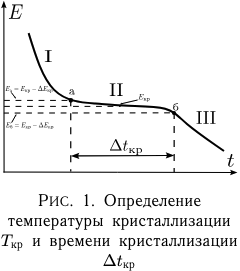
\includegraphics[width=0.4\textwidth]{pick_1} % Placeholder for actual figure
    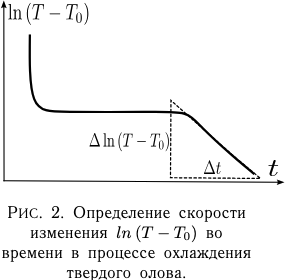
\includegraphics[width=0.4\textwidth]{pick_2} % Placeholder for actual figure
\end{figure}

% \begin{figure}[htbp]
%     \centering
%     \fbox{\parbox[c][5cm][c]{0.45\textwidth}{\centering Placeholder for Figure 2}}
%     \caption{Определение скорости изменения $\ln(T - T_0)$ во времени в процессе охлаждения твердого олова.}
%     \label{fig:graph_lnT_t}
% \end{figure}
%

Для определения коэффициента $K$ необходимо составить для участка III охлаждения олова таблицу значений натурального логарифма $T'$ в зависимости от времени охлаждения $t$, построить график этой зависимости и определить тангенс угла его наклона к оси $t$ (рис. 2). По мере того как разность температур олова и окружающей среды уменьшается, уменьшается и скорость охлаждения олова. Для того, чтобы максимально точно определить коэффициент $K$ нужно выбрать небольшой участок графика – около трех минут после окончания кристаллизации. Погрешность коэффициента $K$ будет определяться погрешностью определения угла наклона графика.

Подставив значения коэффициента $K$, времени кристаллизации $\Delta t_{\text{кр}}$ и температуры кристаллизации $T_{\text{кр}}$ в \eqref{eq:11} и \eqref{eq:12}, вычислим удельную теплоту кристаллизации олова.

Относительные погрешности величин $\lambda$ и $S_2-S_1$ определяются по следующим формулам:
\begin{equation} \label{eq:16}
\frac{\Delta(S_2 - S_1)}{(S_2 - S_1)} = \sqrt{ \left(\frac{\Delta\lambda}{\lambda}\right)^2 + \left(\frac{\Delta M_0}{M_0}\right)^2 + \left(\frac{\Delta T_{\text{кр}}}{T_{\text{кр}}}\right)^2 },
\end{equation}
\begin{equation} \label{eq:17}
\frac{\Delta\lambda}{\lambda} = \sqrt{ \left(\frac{\Delta t_{\text{кр}}}{t_{\text{кр}}}\right)^2 + \left(\frac{\Delta K}{K}\right)^2 + \left(\frac{\Delta T_{\text{кр}}}{T_{\text{кр}} - T_0}\right)^2 }.
\end{equation}
В последней формуле учтено, что вклад погрешностей величин $K, t_{\text{кр}}$ и $T_{\text{кр}}$ значительно превосходят вклады погрешностей $c_0, M_0, c_A, M_A$.

\section*{Экспериментальная установка}

Ампула с оловом 1 (рис. 3) с помощью винта 3 может быть закреплена в двух положениях: в электрической печи 2 или в поднятом состоянии. Внутри ампулы находится металлическая трубка-чехол с хромель-копелевой термопарой 4. Концы термопары соединены с гнездами на штанге стенда 5, которые для выполнения работы необходимо соединить с входными гнездами милливольтметра 6. Подключение электрической печи к сети осуществляется тумблером «нагрев» 7. Тумблер «сеть» 8 служит для подачи напряжения на стенд.

\begin{figure}[htbp]
    \centering
    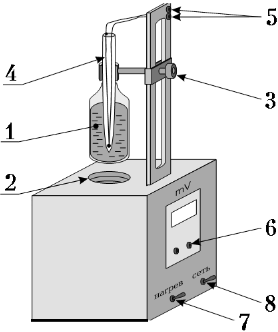
\includegraphics[width=0.7\textwidth]{pick_3} % Placeholder for actual figure
    \caption{Схема экспериментальной установки.}
    \label{fig:setup_schema}
\end{figure}\begin{figure}[H]
\begin{center}
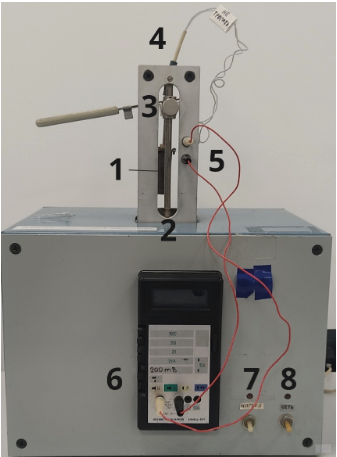
\includegraphics[width=0.6\textwidth]{setup_image.png} % ЗАМЕНИТЕ setup_image.png НА ИМЯ ФАЙЛА С РИСУНКОМ УСТАНОВКИ
\caption{Схема экспериментальной установки: 1 - ампула с оловом, 2 - электрическая печь (нагреватель), 3 - прижимной винт, 4 - термопара в чехле, 5 - штанга стенда с разъемами, 6 - милливольтметр, 7 - тумблер "нагрев", 8 - тумблер "сеть". (Рисунок из методички)}
\label{fig:setup}
\end{center}
\end{figure}

\section{\textbf{Результаты измерений и обработка}}

\subsection{Входные данные и параметры}

\begin{itemize}
    \item Масса олова: $M_o = 0.07 \pm 0.001$ кг
    \item Масса ампулы: $M_A = 0.04 \pm 0.001$ кг
    \item Удельная теплоемкость олова : $c_o = 0.230 \pm 1$  $\frac{\text{кДж}}{\text{кг}\cdot\text{К}}$ 
    \item Удельная теплоемкость ампулы (сталь): $c_A = $ 0.460 $\pm 1$ $\frac{\text{кДж}}{\text{кг}\cdot\text{К}}$
    \item Температура окружающей среды: $T_0 = $ 24.5 $\pm 0.5$ $^{\circ}C$
\end{itemize}

\subsection{Экспериментальные данные}

Зависимость термоЭДС $E$ от времени $t$ при охлаждении олова представлена в таблице \ref{tab:data_E}.

\begin{table}[H]
\centering
\caption{Экспериментальные данные: зависимость термоЭДС от времени.}
\label{tab:data_E}
\sisetup{round-mode=places, round-precision=2} % Округление для таблицы
\begin{tabular}{|c|S[table-format=2.2]||c|S[table-format=2.2]||c|S[table-format=2.2]|}
\hline
{$t$ (\si{\second})} & {$E$ (\si{\milli\volt})} & {$t$ (\si{\second})} & {$E$ (\si{\milli\volt})} & {$t$ (\si{\second})} & {$E$ (\si{\milli\volt})} \\ \hline
0     & 19.90   & 210   & 13.80  & 420   & 11.50  \\ \hline
15    & 18.60   & 225   & 13.60  & 435   & 11.40  \\ \hline
30    & 17.50   & 240   & 13.40  & 450   & 11.20  \\ \hline
45    & 16.60   & 255   & 13.20  & 465   & 11.10  \\ \hline
60    & 15.90   & 270   & 13.00  & 480   & 11.00  \\ \hline
75    & 15.40   & 285   & 12.80  & 495   & 10.80  \\ \hline
90    & 15.10   & 300   & 12.70  & 510   & 10.70  \\ \hline % Начало плато
105   & 15.10   & 315   & 12.50  & 525   & 10.60  \\ \hline
120   & 15.10   & 330   & 12.40  & 540   & 10.50  \\ \hline
135   & 15.10   & 345   & 12.20  & 555   & 10.40  \\ \hline
150   & 15.10   & 360   & 12.10  & 570   & 10.20  \\ \hline
165   & 15.10   & 375   & 12.00  & 585   & 10.10  \\ \hline % Конец плато
180   & 14.80   & 390   & 11.80  & 600   & 10.00  \\ \hline
195   & 14.40   & 405   & 11.70  & \multicolumn{2}{c|}{}        \\ \hline % Убрана пустая ячейка
\end{tabular}
\end{table}

График зависимости ЭДС от времени $E(t)$ представлен на рис. \ref{fig:graph_E_t}.


\begin{figure}[H]
\centering
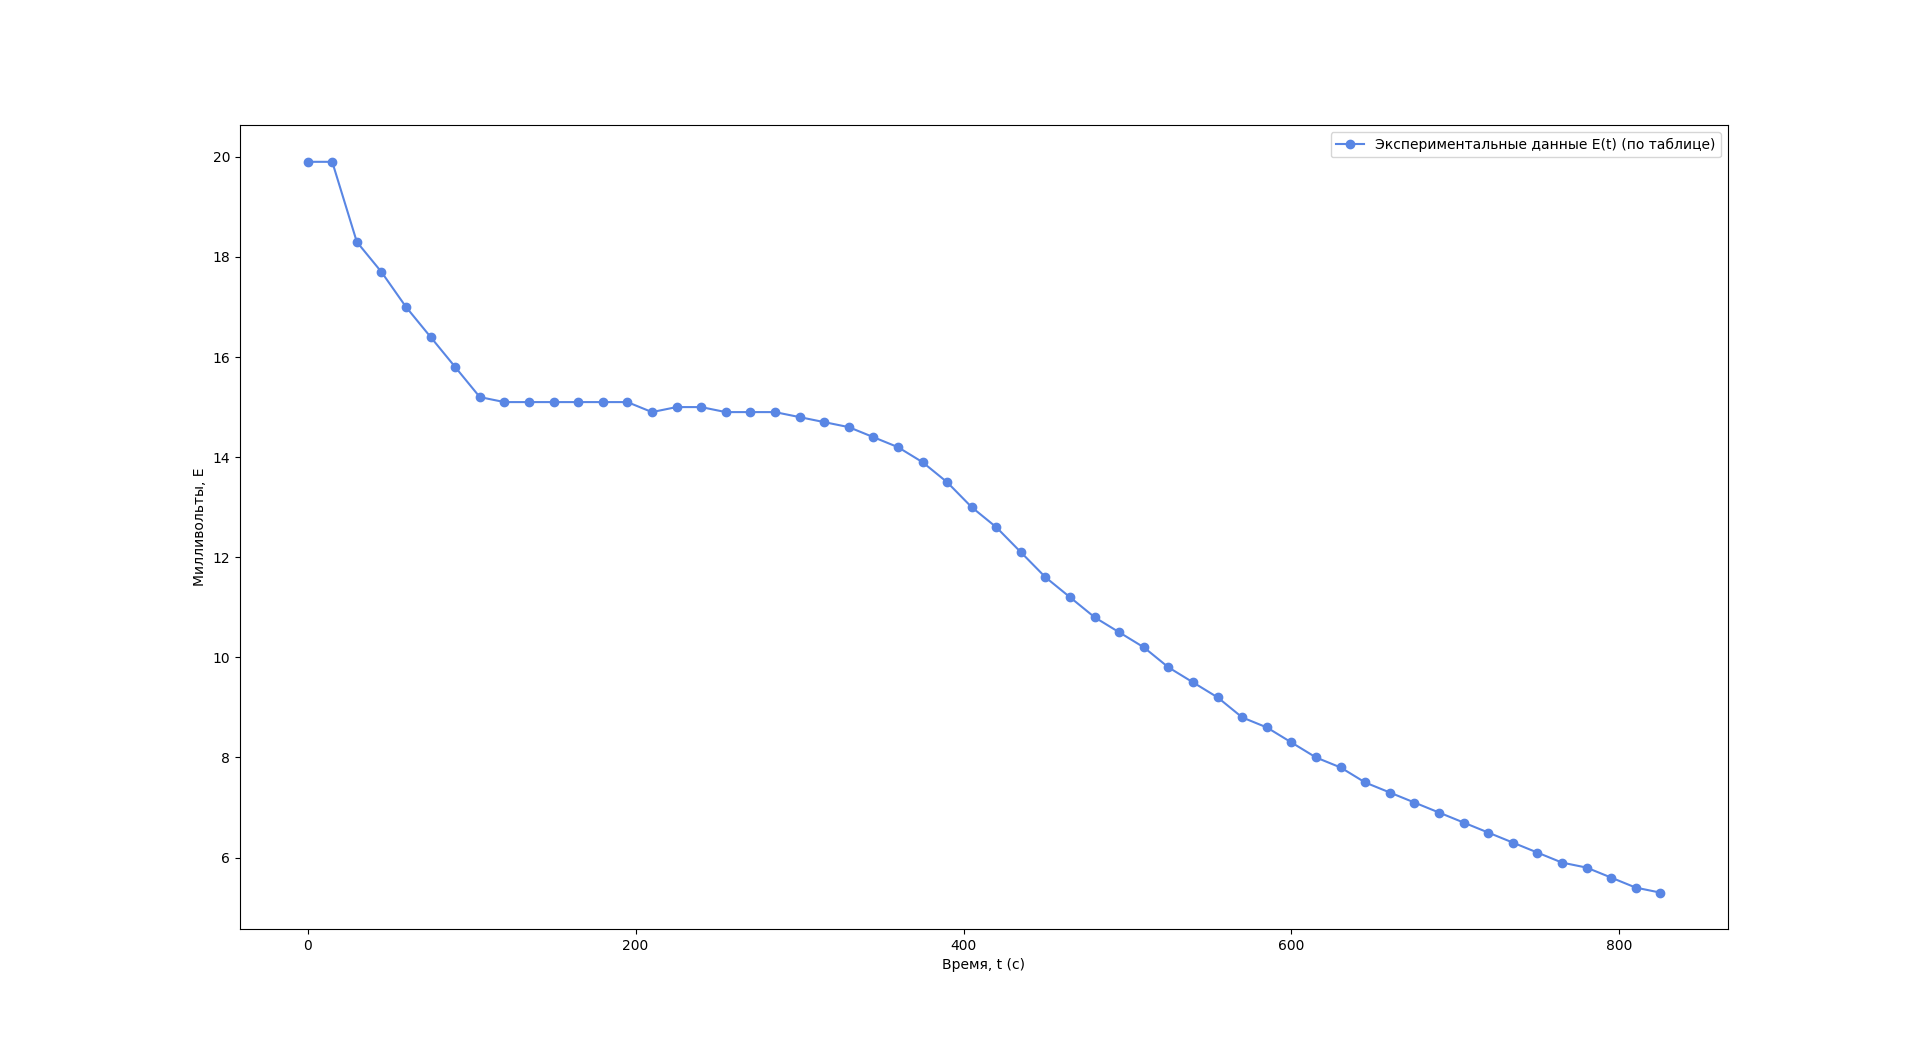
\includegraphics[width=0.9\textwidth]{fig_3} % ЗАМЕНИТЕ graph_E_t.png НА ИМЯ ФАЙЛА С ГРАФИКОМ E(t)
\caption{График зависимости термоЭДС от времени при охлаждении олова. Участки: I - охлаждение жидкости, II - кристаллизация, III - охлаждение твердого тела.}
\label{fig:graph_E_t}
\end{figure}

График зависимости T от времени $T(t)$ представлен на рис. \ref{fig:graph_T_t}.
\begin{figure}[H]
\centering
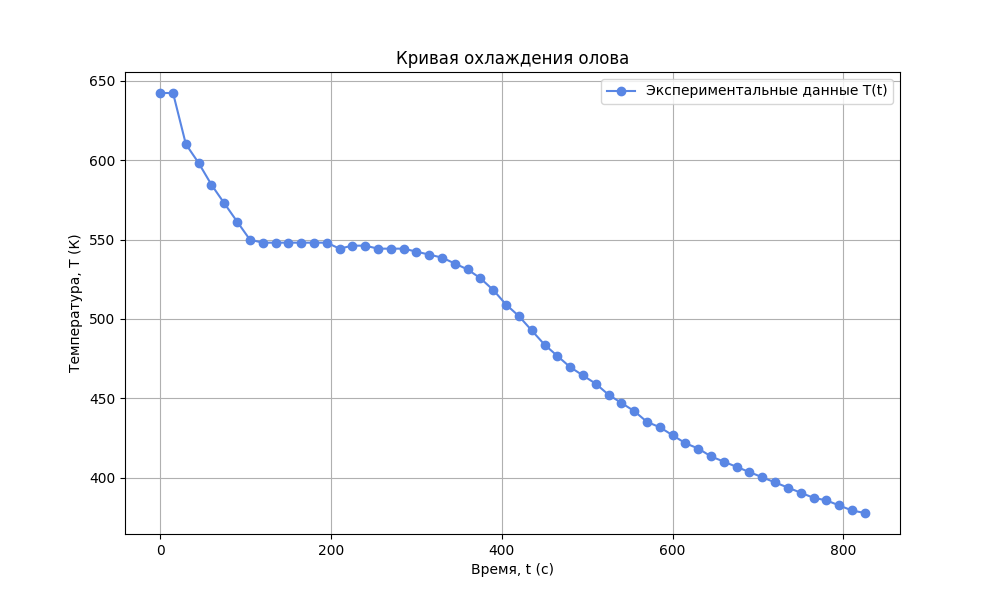
\includegraphics[width=0.9\textwidth]{fig_1} % ЗАМЕНИТЕ graph_E_t.png НА ИМЯ ФАЙЛА С ГРАФИКОМ E(t)
\caption{График зависимости термоЭДС от времени при охлаждении олова. Участки: I - охлаждение жидкости, II - кристаллизация, III - охлаждение твердого тела.}
\label{fig:graph_T_t}
\end{figure}

\subsection{Определение параметров кристаллизации}

Из графика $E(t)$ и таблицы \ref{tab:data_E} определяем параметры плато кристаллизации (участок II):
\begin{itemize}
    \item ЭДС кристаллизации: $E_{кр} = \SI{15.10}{\milli\volt}$. (Среднее значение на плато). Погрешность ЭДС примем $\pm \SI{0.05}{\milli\volt}$ (половина последнего значащего разряда или по паспорту прибора).
    \item Начало кристаллизации: $t_{нач} \approx \SI{110}{\second}$.
    \item Конец кристаллизации: $t_{кон} \approx \SI{380}{\second}$.
    \item Время кристаллизации: $\Delta t_{кр} = t_{кон} - t_{нач} = \SI{380}{\second} - \SI{110}{\second} = \SI{270}{\second}$.
    Погрешность определения границ плато $\approx \pm \SI{7.5}{\s}$ (половина интервала). Погрешность $\Delta t_{кр} \approx \sqrt{7.5^2 + 7.5^2} \approx \SI{10.6}{\s}$.
\item Температура кристаллизации $T_{\text{кр}} = 231.0 \pm 0.5 $ $^{\circ}C$.
\end{itemize}

\subsection{Определение коэффициента охлаждения K}

Для определения коэффициента $K$ используем данные участка III (охлаждение твердого олова, $t > \SI{165}{\s}$). Необходимо перевести ЭДС $E$ в температуру $T = T' + T_0$, где $T'$ (разность температур) находится по таблице термопары. Затем строится график зависимости $\ln(T - T_0) = \ln(T')$ от времени $t$.

\begin{table}[H]
\centering
\caption{Данные для расчета коэффициента K (Участок III).}
\label{tab:data_K}
\sisetup{round-mode=places, round-precision=2}
\begin{tabular}{|c|S[table-format=2.2]|c|c|S[table-format=1.2]|}
\hline
{$t$ (\si{\second})} & {$E$ (\si{\milli\volt})} & {$T'$ (\si{\celsius})} & {$T = T'+T_0$ (\si{\kelvin})} & {$\ln(T')$} \\ \hline
180 & 14.80 & 202.7 & 500.3 & 5.31 \\ \hline % T' и ln(T') взяты из данных Python (приблизительно)
195 & 14.40 & 197.5 & 495.1 & 5.29 \\ \hline
210 & 13.80 & 189.9 & 487.5 & 5.25 \\ \hline
% ... (добавьте больше точек из вашего расчета T') ...
480 & 11.00 & 151.1 & 448.7 & 4.98 \\ \hline
% ...
600 & 10.00 & 137.2 & 434.8 & 4.92 \\ \hline
\end{tabular}
\end{table}

График зависимости $\ln(T - T_0)$ от $t$ представлен на рис. \ref{fig:graph_lnT_t}.

\begin{figure}[H]
\centering
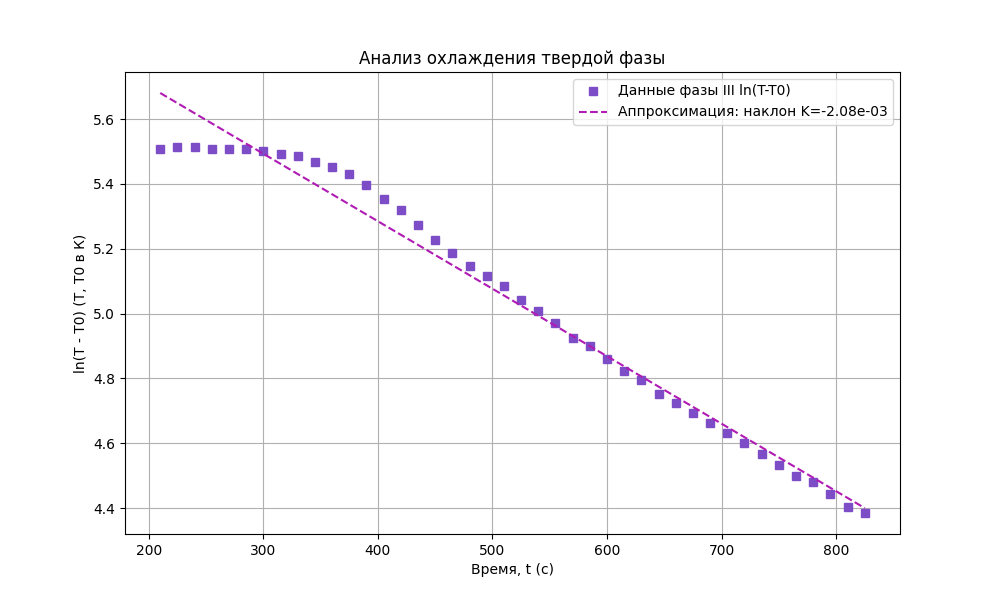
\includegraphics[width=0.9\textwidth]{fig_2} % ЗАМЕНИТЕ graph_lnT_t.png НА ИМЯ ФАЙЛА С ГРАФИКОМ ln(T-T0) от t
\caption{График зависимости натурального логарифма разности температур $\ln(T - T_0)$ от времени $t$ для участка охлаждения твердого олова. Прямая линия - линейная аппроксимация.}
\label{fig:graph_lnT_t}
\end{figure}

Коэффициент $K$ равен модулю тангенса угла наклона аппроксимирующей прямой.
$K = {2.0800e-3 \pm 0.0434e-3}$.

\subsection{Расчет удельной теплоты кристаллизации $\lambda$}

Используем формулу :
$\lambda = (c_o + c_A \frac{M_A}{M_o}) K (T_{кр} - T_0) \Delta t_{кр}$
$\lambda = \left(\SI{230}{\joule\per\kilo\gram\per\kelvin} + \SI{460}{\joule\per\kilo\gram\per\kelvin} \times \frac{\SI{0.04000}{\kilo\gram}}{\SI{0.07027}{\kilo\gram}}\right) \times (\SI{2.0800e-3}{\per\second}) \times (\SI{504.15}{\kelvin} - \SI{297.65}{\kelvin}) \times (\SI{270}{\second})\approx 51.8 \pm 10.4$


Литературное значение: $\lambda_{лит} = \SI{60.7}{\kilo\joule\per\kilo\gram}$.

\subsection{Расчет изменения энтропии}

Удельное изменение энтропии по формуле :
$\Delta s = -\frac{\lambda}{T_{кр}} = -\frac{51.8e3}{504.15} \approx \SI{-102.75}{\text{дж}\per\kilo\gram\cdot\kelvin}$.

Полное изменение энтропии образца олова:
$\Delta S = \Delta s \times M_o = -102.65\times 0.07027 \approx \SI{-7.213}{\text{дж}\per\kelvin}$.

\subsection{Оценка погрешностей}

Относительная погрешность $\lambda$ (формула (17) из методички):
$\frac{\Delta \lambda}{\lambda} = \sqrt{ \left(\frac{\Delta (\Delta t_{кр})}{\Delta t_{кр}}\right)^2 + \left(\frac{\Delta K}{K}\right)^2 + \left(\frac{\Delta (T_{кр}-T_0)}{T_{кр}-T_0}\right)^2 }$
$\frac{\Delta \lambda}{\lambda} = \sqrt{ \left(\frac{15}{75}\right)^2 + \left(\frac{0.0434e-3}{2.0800e-3}\right)^2 + \left(\frac{\sqrt{\Delta T_{кр}^2 + \Delta T_0^2}}{T_{кр}-T_0}\right)^2 }$
$\frac{\Delta \lambda}{\lambda} = \sqrt{ (0.2)^2 + (0.0208)^2 + \left(\frac{\sqrt{0.5^2 + 0.5^2}}{206.5}\right)^2 }$
$\frac{\Delta \lambda}{\lambda} = \sqrt{ 0.04 + 0.00043 + (\frac{0.707}{206.5})^2 } \approx \sqrt{ 0.04 + 0.00043 + (0.0034)^2 } \approx \sqrt{0.04044} \approx 0.201$
Абсолютная погрешность $\Delta \lambda = \lambda \times 0.201 = 51.8\times 0.201 \approx 10.4$.

Относительная погрешность $\Delta S$:
$\frac{\Delta (\Delta S)}{|\Delta S|} = \sqrt{ \left(\frac{\Delta \lambda}{\lambda}\right)^2 + \left(\frac{\Delta M_0}{M_0}\right)^2 + \left(\frac{\Delta T_{кр}}{T_{кр}}\right)^2 }$
$\frac{\Delta (\Delta S)}{|\Delta S|} = \sqrt{ (0.201)^2 + \left(\frac{0.01}{70.27}\right)^2 + \left(\frac{0.5}{504.15}\right)^2 }$
$\frac{\Delta (\Delta S)}{|\Delta S|} \approx \sqrt{ 0.0404 + (0.00014)^2 + (0.00099)^2 } \approx \sqrt{0.0404} \approx 0.201$
Абсолютная погрешность $\Delta (\Delta S) = |\Delta S| \times 0.201 = \SI{7.213}{\joule\per\kelvin} \times 0.201 \approx \SI{1.45}{\joule\per\kelvin}$.

\section{\textbf{Вывод}}

В ходе лабораторной работы была исследована кристаллизация олова как фазовый переход первого рода. На основе экспериментальных данных охлаждения расплава олова были получены: 
\begin{enumerate}
\item Значения $T_{кр}$ и $\lambda$, которые согласуются с табличными в рамках погрешностей эксперимента. 
\item Подтверждено уменьшение энтропии при кристаллизации. 
\end{enumerate}
Погрешности измерений оказались в пределах допустимых значений, что позволяет сделать вывод о корректности проведенного эксперимента и приминимости теории. Погрешность могла получится из-за принятия $\Delta t = 270$, так как это число было взято на глаз из графика, отсюда и погрешность. 

\end{document}

В ходе выполнения работы 2.4 была исследована зависимость коэффициента внутреннего трения от размеров объекта. Полученные результаты о независимости коэффициента внутреннего трения от размеров объекта согласуются с теорией. Погрешности измерений оказались в пределах допустимых значений, что позволяет сделать вывод о корректности проведенного эксперимента и приминимости теории. Погрешность может быть вызвана не точностью измерения времени, так как человек не сразу нажимает на секундомер. 
Результаты на больших шариках получились лучше, так как они менее чувствительны к неоднородности среды, те меньше влияние внешних факторов.
